\documentclass[conference]{IEEEtran}
\usepackage[T1]{fontenc}
\usepackage{graphicx}
\usepackage{booktabs}
\usepackage{amsmath}
\usepackage{url}
\usepackage[hidelinks]{hyperref}
\usepackage{xcolor}

\newcommand{\dash}{--}

\begin{document}

\title{Everfold: Do Generative World Models Give\\Two Players the Same World?}

\author{\IEEEauthorblockN{Wanzhen Jiang}
\IEEEauthorblockA{Independent Researcher\\
wjiang88@alumni.stanford.edu}}

\maketitle

\begin{abstract}
Generative world models are pitched as future game engines, and studios are testing them as renderers. Their public evaluations are single-player: one viewer, one camera. A multiplayer game needs more. Two players looking at the same tower must see the same tower, and when one player fells a tree, the other must see the stump. We present Everfold, an open multiplayer test world with an authoritative game server, and a benchmark of five probes that score a renderer's frames against the server's ground truth: cross-view agreement, revisit retention, cross-player state propagation, identity persistence, and shared-structure state change. A blind vision-language judge reads the frames; two human labellers check it, and at the level the scores use it agrees with each of them as often as they agree with each other (41--42 of 46 probe decisions). We test five ways of putting a generative model into a game, over 20 seeds where cost allowed: hosted realtime world models that hold their own state, a game-locked world model, a stateless text-to-image renderer, a video restyler over the server's 3D render, and the server's own render. No realtime world model propagates a state change (0--2\%), and given one session per player, none shows the two players the same landmark more than 10\% of the time. Restyling the server's geometry raises this to 35\%; the server's own render reaches 100\%. Consistency follows whoever holds a single shared state. Whether a generative model can hold that state and update it for several players, as a persistent generated world or as a learned simulator, is the open question Everfold is built to test.
\end{abstract}

\begin{IEEEkeywords}
world models, multiplayer games, benchmark, generative rendering, evaluation
\end{IEEEkeywords}

\section{Introduction}

Live world models such as Google DeepMind's Genie~4 and Runway's GWM-1 Worlds generate frames as the user steers. Genie~4 also generates sound and talking characters, and creatives are testing it as a ``draft mode'' for previsualisation~\cite{genie4}. DeepMind's own announcement says visual details and object permanence can drift in longer sessions and after several prompt edits~\cite{genie4}. Runway claims that returning to an earlier position restores the same view~\cite{gwm1}. These claims come from vendors, and they concern one viewer.

Games are rarely one viewer. In any shared world, two players at the same moment must see one consistent state: the same buildings, the same people in the same clothes, and the consequences of each other's actions. Two routes are being tried for a generative model to provide that. One generates a persistent 3D world once, as World Labs' Marble does~\cite{marble}. The other learns the simulation itself and renders it per player, as Odyssey's Agora-2~\cite{agora2} and MASS~\cite{mass} propose. Recent multiplayer world models are each evaluated on their own game and their own terms (Section~\ref{sec:related}). No benchmark asks different kinds of model the same multiplayer questions against an authoritative ground truth.

We contribute:
\begin{enumerate}
\item \textbf{Everfold}, an open real-time multiplayer world with an authoritative server, chunked procedural terrain, villagers and quests written on demand by a language model, two-player shrines, and a pluggable renderer interface.
\item \textbf{Five multiplayer probes} with server ground truth, a blind vision judge validated against two human labellers, and a pair judge for cross-view consistency with positive and negative controls.
\item \textbf{Results across five integration patterns}: hosted realtime world models, a game-locked world model, a stateless text-to-image renderer, a video restyler over the server's 3D render, and the server render itself, with cost and latency.
\item \textbf{A grounding measure for generated content}: how often quests written by a language model point at things that do not exist, and where such inventions enter.
\end{enumerate}

\section{Related Work}\label{sec:related}

\emph{Generative game engines and world models.} Diffusion models can stand in for a game's renderer and simulation at interactive rates: GameNGen for DOOM~\cite{gamengen}, DIAMOND for Atari~\cite{diamond}, and Oasis for Minecraft~\cite{oasis}. Genie learned controllable environments from video~\cite{genie}; its successors, Genie~3~\cite{genie3} and Genie~4~\cite{genie4}, explore open-ended worlds in real time. Marble~\cite{marble} instead generates a persistent, explorable 3D world (Gaussian splats and a mesh) from text, images or video.

\emph{Single-player world-model benchmarks} test one viewer. WorldScore~\cite{worldscore} scores camera-controlled world generation. WorldRoamBench~\cite{worldroam} and MIND~\cite{mind} test action following, drift and revisit memory.

\emph{Multiplayer world models} are new, and each is tested on its own terms. Solaris~\cite{solaris} is an open two-player Minecraft model with view-consistency metrics. MultiGen~\cite{multigen} adds shared editable memory in Doom. WorldCast~\cite{worldcast} runs per-player generators that exchange state in Counter-Strike~2. Multiverse~\cite{multiverse} is a two-player split-screen racing model. MIRA~\cite{mira} renders four synchronised views of Rocket League 2v2 from one shared latent. Agora-2~\cite{agora2} pairs a learned simulation model with one renderer per player; its report notes that view agreement and latency were not measured. MASS~\cite{mass} separates a learned logic engine from per-player rendering, evaluated on Snake. PROWL-2~\cite{prowl2} trains agents inside a world model, gated by fidelity to recorded trajectories.

Everfold differs in two ways. It holds a real game's state in a server and scores renderers against it, so heterogeneous systems answer the same questions. And it treats the renderer as replaceable, following World Labs' functional taxonomy of world models as renderers, simulators and planners~\cite{taxonomy}.

\section{Everfold}

\textbf{World.} Everfold is an endless, seeded world of 32$\times$32-tile chunks. Ground types include meadow, forest, river and village square. Features include trees, bushes, rocks, houses, wells and chests. Landmarks are villages, ruins, stables, watchtowers crowned with a blue flame, and shrines with two pressure plates. A shrine's gate opens only while two players stand on its plates, so strangers must cooperate. Players can fell trees (leaving stumps), light campfires and gather items. An authoritative server holds all state; the browser client and every renderer only display it. Throughout, \emph{engine} means this server: the game's own code, written for this study, that holds the true world and applies the rules. It is not a commercial engine such as Unity or Unreal; in the benchmark it is the referee that knows the right answers. Villagers' personalities and quests are written on demand by a language model and checked against the real world before a player sees them (Section~\ref{sec:grounding}).

\textbf{Views and prompts.} For any player, the engine computes what the camera should see: the ground underfoot, landmarks, people and features in a 100$^\circ$ cone, with side and distance. It compiles that view into a fixed-order prompt: the player's look, the land ahead, people, what changed, the camera, then a fixed art direction. It also produces short checkable claims, for example ``a tree stump is visible''. Every person has a fixed outfit (colour and garment) and a carried item, so identity is checkable.

\textbf{Greybox.} The engine also renders the true state in 3D: flat ground tiles, boxes for trees, houses and people, a stone column with a blue flame for a tower. It uses a high third-person chase camera over the player's shoulder, and fades tall occluders in the line of sight, as games do. This is the engine's blockout pass. It is a reference renderer, and the input that the restyling model receives.

\section{Benchmark}

\textbf{Probes.} Each probe scripts bench players through the real engine and snapshots the true state at every step (14 steps per seed):
\begin{itemize}
\item \emph{Cross-view}: two players look at one watchtower from different sides. Score: does each frame show the tower?
\item \emph{Same tower} (cross-view consistency): a pair judge sees both players' frames together. Score: is it recognisably the same structure from two sides?
\item \emph{Revisit}: a player looks at a village, walks away facing elsewhere, then returns to the first pose. Score: the share of landmarks, people and features first shown that appear again.
\item \emph{Propagation}: one player fells a tree, then lights a campfire, while a second player watches. Score: per transition, the frame before must show the old state and not the new one, and the frame after the reverse. A picture that never changes cannot pass.
\item \emph{Identity}: one player is seen by another from three poses over time. Score: is the player, identified by outfit, shown each time?
\item \emph{Shrine}: two players open a shrine while a third watches (sealed gate, then open gate and spirit orb). Scored per transition, like propagation.
\end{itemize}

Probes that need the camera to move are not scored (n/a) when the camera did not move. That is detected two ways: consecutive frames correlating above 0.9 on normalised thumbnails, or the pair judge answering that the second cross-view frame was taken from the same spot. The second check applies only where the model controls its own camera.

\textbf{Judge.} A vision-language model (Claude Opus 5.5) sees one frame and a numbered list of claims, never the prompt. The list includes claims that are no longer true (the state before a change), unmarked. It answers present, absent or unclear for each. Multimodal model judges can diverge from human judgement~\cite{mllmjudge}, so we validate this one against people.

After the first multi-seed round, three claims were loosened. The justification came only from the stateless oracle (Section~\ref{sec:results}), which failed them on frames drawn from the true state, not from any world model's scores: ``a tree stump'', not ``a fresh tree stump'', because clearly drawn weathered stumps were rejected; the shrine as its platform alone, with its gate and plates already separate facts; and people by outfit only. Every saved frame was re-judged with the new wording. No conclusion changes: the world models' state-change scores stay at 0--2\% under either wording, while the oracle's propagation rises from 30\% to 82\%.

\textbf{Human agreement.} Two labellers answered the same question blind, on 50 frames (319 claims) sampled across five conditions and weighted toward the changed claims. Neither saw the judge's answers. The first labeller knew the study design; the second worked only from a one-page brief (Table~\ref{tab:agree}).

\begin{table}[t]
\caption{Agreement on 50 frames (319 claims).}\label{tab:agree}
\centering
\begin{tabular}{@{}lccc@{}}
\toprule
Pair & Present $\kappa$ & People $\kappa$ & Probe pass/fail \\
\midrule
Human 1 vs Human 2 & 0.82 & 0.71 & 41/46 \\
Human 1 vs judge & 0.66 & 0.53 & 41/46 \\
Human 2 vs judge & 0.65 & 0.58 & 42/46 \\
\bottomrule
\end{tabular}
\end{table}

The judge is noisier than a second person on single claims, especially clothing, but its disagreements run both ways, so it is not biased. At the level the probe scores use, it agrees with each human as often as the humans agree with each other. An earlier round of 98 frames gave $\kappa = 0.74$. The pair judge was tested with controls: a tower and a mirrored, cropped copy of itself were judged the same 20 of 20 times, and two independently drawn towers 3 of 19 times.

\textbf{Conditions.} Table~\ref{tab:conditions} lists the five integration patterns.

\begin{table*}[t]
\caption{Conditions, grouped by who holds the world state.}\label{tab:conditions}
\centering
\begin{tabular}{@{}p{3.6cm}p{4.2cm}p{9.0cm}@{}}
\toprule
Pattern & Condition & What it is \\
\midrule
Model holds state & ABot-World-0~\cite{abot}, LingBot-World-2~\cite{lingbot} (fal realtime) & Text-steered streaming world models. Start image generated from the first prompt; prompt updates per step. \emph{Drive}: one session walked between poses with movement commands. \emph{Image only}: prompts alone. \emph{Per player}: one session per player. \\
Game-locked & Eden Live 14B Game~\cite{eden} & A world model that always runs one of its built-in games. \\
Stateless renderer & FLUX.1 schnell~\cite{flux} (``oracle'') & Each frame drawn fresh from the true-state prompt; no memory to lose. \\
Engine renders, model restyles & Decart Lucy Restyle~\cite{lucy} (offline video-to-video) & Restyles one greybox clip per probe family (held at each pose, walking between them), or one clip per player. \\
Engine renders & Greybox & The engine's own 3D render. \\
\bottomrule
\end{tabular}
\end{table*}

\section{Results}\label{sec:results}

\begin{table*}[t]
\caption{Probe scores, mean over seeds with 95\% bootstrap intervals (seed is the unit). Seeds: 20, except LingBot drive 12.}\label{tab:results}
\centering
\begin{tabular}{@{}lcccccc@{}}
\toprule
Condition & Cross-view & Same tower & Revisit & Propagation & Identity & Shrine \\
\midrule
ABot, drive & 0\% & 0\% & 15\% [5, 27] & 2\% [0, 8] & 13\% [5, 22] & 0\% \\
LingBot, drive & 9\% [0, 27] & 0\% & 19\% [7, 32] & 0\% & 22\% [8, 36] & 0\% \\
ABot, per player & 75\% [55, 90] & 5\% [0, 15] & -- & -- & -- & -- \\
LingBot, per player & 80\% [60, 95] & 10\% [0, 25] & -- & -- & -- & -- \\
FLUX oracle & 95\% [84, 100] & 16\% [0, 32] & 89\% [80, 96] & 82\% [72, 92] & 37\% [22, 52] & 30\% [10, 50] \\
Lucy, one clip & 40\% [20, 60] & 10\% [0, 25] & 0\% ($n{=}6$) & 0\% & 10\% [3, 18] & 0\% \\
Lucy, per player & 80\% [60, 95] & 35\% [15, 55] & -- & -- & -- & -- \\
Greybox & 100\% & 100\% & 99\% [97, 100] & 0\%$^{*}$ & 70\% [57, 83] & 20\% [5, 40] \\
\bottomrule
\end{tabular}

\vspace{2pt}
\begin{minipage}{0.95\textwidth}\footnotesize
$^{*}$The player who fells the tree stands between the watcher and the stump; the probes' text truth has no occlusion, a true 3D camera does.
\end{minipage}
\end{table*}

\begin{figure}[t]
\centering
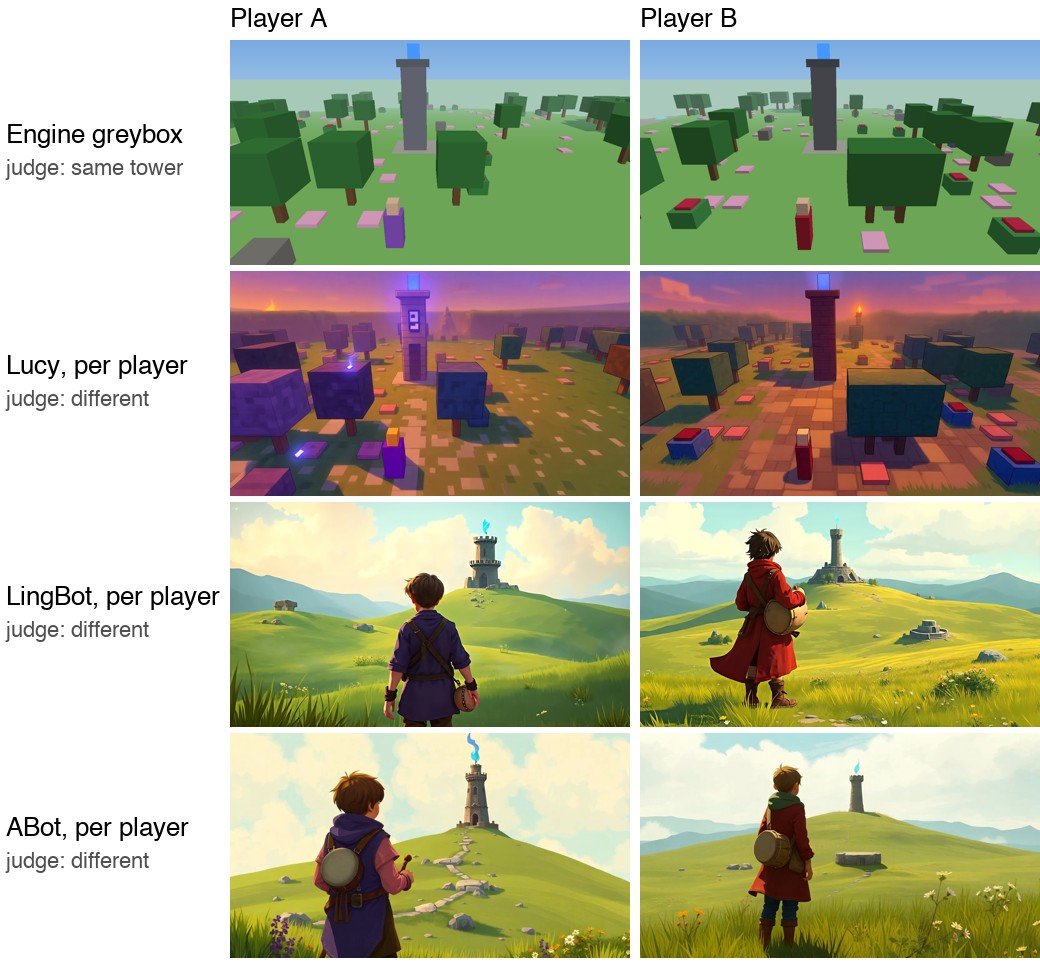
\includegraphics[width=\columnwidth]{fig1-cross-view.jpg}
\caption{One tower, two players, four renderers (seed 3), with the pair judge's verdict. Only the engine render gives both players the same tower; each per-player model draws its own.}
\label{fig:crossview}
\end{figure}

Table~\ref{tab:results} gives the scores and Fig.~\ref{fig:crossview} an example.

\textbf{No world model propagates a state change.} When one player fells a tree or opens a shrine, the other player's view never shows it (0--2\% across 32 driven seeds). The stateless oracle, told the true state each frame, manages 82\% on propagation, so the claims are drawable. The gap is memory and prompt following, not wording.

\textbf{No realtime world model gives two players one world.} Walked between the two viewpoints, one session loses the tower (0--9\%). Given one session each, both players see a tower (75--80\%), each drawn from its own start image, but almost never the same one (5--10\%). The oracle reaches only 16\% for the same reason: independent frames share no world.

\textbf{Restyling shared geometry helps, but only partly.} Lucy keeps the engine's layout but recolours freely (purple trees), invents effects (fire, glows), and drifts over long clips. Given one clip per player, it shows the same tower 35\% of the time. The ordering is the paper's main result: one shared state (the engine render, 100\%), then a model restyling shared geometry per player (35\%), then a model inventing the world per player (5--10\%). Consistency is lost exactly where each player's renderer is free to invent.

\textbf{Without movement commands the camera does not move.} Steered by prompts alone, ABot and LingBot return a near-identical frame after 81--85\% of moves. Pose probes are then untestable, which is why we drive them.

\textbf{A game-locked model cannot carry the probes.} Eden always runs one of its 12 built-in games. Under its default game it drops the game's props into our scene, then stops moving the camera: frames before and after a turn correlate at 0.98--0.99. Under its free-flight game, the camera moves, but within four seconds the scene becomes the game's own forest. We report it qualitatively, from 3 seeds and a controls test.

\textbf{Robustness.} Scaling the drive calibration by $\times$0.5 and $\times$1.5 leaves state changes and same tower at 0\% (5 seeds each). fal refused or never confirmed 7.8\% of prompt updates (56 of 714), some for content moderation. Rescoring only refusal-free runs changes no conclusion.

\section{Content Grounding}\label{sec:grounding}

Quests are written by a language model from a context listing real places, people and items by id, then validated before a player sees them. Across 20 worlds (57 quests, Claude Opus 5.5 at the game's low effort setting), 0 of 200 quest steps pointed at anything that does not exist, and no quest named an invented place or person. But 49\% of quests (28 of 57) asked for an item variety the game does not have, such as ``glowcap moss'' or ``silverbell'', which the step quietly maps to a generic herb or mushroom. All 28 trace to the villager's own want, written one stage earlier by the persona generator: invention enters upstream and propagates. With fixed, scripted personalities instead, no item was invented, but variety collapsed: one title recurred 19 times in 60 quests. Grounding and variety trade off through the persona stage.

\section{Cost and Latency}

\begin{table}[t]
\caption{Price and latency of each renderer.}\label{tab:cost}
\centering
\footnotesize
\begin{tabular}{@{}p{1.55cm}p{2.15cm}p{3.75cm}@{}}
\toprule
Renderer & Price & Latency \\
\midrule
ABot, LingBot & \$4.50 / player-hour & acknowledged 1.8 / 3.9\,s; picture changes 1.8 / 1.6\,s \\
Eden & \$36 / player-hour & acknowledged 1.3\,s; picture changes 3.4\,s \\
Lucy (fal) & \$0.01 / video second & batch, not realtime \\
FLUX schnell & \$0.003 / image & 1.5\,s per frame \\
Greybox & free & instant \\
\bottomrule
\end{tabular}
\end{table}

Table~\ref{tab:cost} compares costs. The whole study (184 judged runs, 1,855 judged frames) cost about \$55 in renderer fees.

\section{Discussion and Limitations}

The results point one way: \textbf{the property a multiplayer game needs, one shared world, comes from whoever holds a single shared state.} Models that hold their own state invent a world per session, and no prompt brings two sessions into agreement. A renderer conditioned on the engine's geometry inherits some of the engine's consistency, and loses it to the extent the model is free to repaint.

That leaves the question the field is betting on. A game needs one state that is shared \emph{and} changes with every player's action. Today that state lives in an engine. Two routes aim to move it into a model: a persistent world generated once and shared by all players, as Marble generates, and a learned simulator with per-player renderers, as in Agora-2 and MASS. Neither is evaluated here, and the reports of the latter do not yet measure view agreement or cross-player propagation. Everfold measures exactly these, against a referee that knows the answers. For a studio shipping today, the practical reading is to keep the game's own state authoritative and constrain any generative model to it as tightly as possible.

\textbf{Limitations.} The probe truth is text-like and ignores occlusion, which penalises true 3D renderers (greybox propagation). The judge is moderately reliable on people ($\kappa$ 0.53--0.58) and not perfectly repeatable, so identity scores carry wider error than the others. Hosted models change without notice and refuse some prompts; Lucy on fal fails silently on prompts over about 900 characters, and we capped ours. Odyssey's models, Genie~3/4 and GWM-1 were not available to us programmatically, World Labs' Marble is not yet included, and open models (Solaris, Matrix-Game) need GPU hosting. These are the next conditions; an Odyssey adapter and a hand-capture path are in place.

\section{Conclusion}

Everfold asks generative models the questions a multiplayer game depends on, against an engine that knows the answers. Today's realtime world models fail them in ways single-player benchmarks cannot see. The benchmark, the world, the labels and every frame are released to make the comparison repeatable as models change.\footnote{Code: \url{https://github.com/jwz8819/everfold}. Frames, judge verdicts and human labels: \url{https://huggingface.co/datasets/jwz8819/everfold-bench}.}

\begin{thebibliography}{99}
\bibitem{genie4} R.~Hadsell, D.~Rivas, and H.~Qi, ``Genie 4: A new generation of world simulation,'' Google DeepMind Blog, Oct. 27, 2026. [Online]. Available: \url{https://deepmind.google/blog/genie-4-a-new-generation-of-world-simulation/}
\bibitem{gwm1} Runway, ``Introducing GWM-1,'' Runway Research, Dec. 11, 2025. [Online]. Available: \url{https://runway.com/research/introducing-runway-gwm-1}
\bibitem{marble} World Labs, ``Marble: A multimodal world model,'' World Labs Blog, Nov. 12, 2025. [Online]. Available: \url{https://www.worldlabs.ai/blog/marble-world-model}
\bibitem{agora2} J.~Grieve \emph{et al.}, ``Agora-2: An action-conditioned world model for real-time multiplayer environments,'' Odyssey, Tech. Rep., Sep. 2026. [Online]. Available: \url{https://agora-2.odyssey.systems/agora-2.pdf}
\bibitem{mass} Z.~Cai \emph{et al.}, ``MASS: Multiplayer world models with authoritative shared state,'' arXiv:2608.06257, 2026.
\bibitem{gamengen} D.~Valevski, Y.~Leviathan, M.~Arar, and S.~Fruchter, ``Diffusion models are real-time game engines,'' in \emph{Proc. ICLR}, 2025, arXiv:2408.14837.
\bibitem{diamond} E.~Alonso, A.~Jelley, V.~Micheli, A.~Kanervisto, A.~Storkey, T.~Pearce, and F.~Fleuret, ``Diffusion for world modeling: Visual details matter in Atari,'' in \emph{Proc. NeurIPS}, 2024, arXiv:2405.12399.
\bibitem{oasis} Decart and Etched, ``Oasis: A universe in a transformer,'' Oct. 31, 2024. [Online]. Available: \url{https://oasis-model.github.io/}
\bibitem{genie} J.~Bruce \emph{et al.}, ``Genie: Generative interactive environments,'' in \emph{Proc. ICML}, 2024, arXiv:2402.15391.
\bibitem{genie3} J.~Parker-Holder and S.~Fruchter, ``Genie 3: A new frontier for world models,'' Google DeepMind Blog, Aug. 5, 2025.
\bibitem{worldscore} H.~Duan, H.-X.~Yu, S.~Chen, L.~Fei-Fei, and J.~Wu, ``WorldScore: A unified evaluation benchmark for world generation,'' in \emph{Proc. ICCV}, 2025, arXiv:2504.00983.
\bibitem{worldroam} T.-B.~Xu \emph{et al.}, ``WorldRoamBench: An open-world benchmark for long-horizon stability of interactive world models,'' arXiv:2606.31672, 2026.
\bibitem{mind} Y.~Ye \emph{et al.}, ``MIND: Benchmarking memory consistency and action control in world models,'' arXiv:2602.08025, 2026.
\bibitem{solaris} G.~Savva \emph{et al.}, ``Solaris: Building a multiplayer video world model in Minecraft,'' arXiv:2602.22208, 2026.
\bibitem{multigen} R.~Po, D.~J.~Zhang, A.~Hertz, G.~Wetzstein, N.~Wadhwa, and N.~Ruiz, ``MultiGen: Level-design for editable multiplayer worlds in diffusion game engines,'' arXiv:2603.06679, 2026.
\bibitem{worldcast} Z.~Ye \emph{et al.}, ``WorldCast: Distributed multiplayer world models,'' arXiv:2610.12412, 2026.
\bibitem{multiverse} Enigma Labs, ``Introducing Multiverse: The first AI multiplayer world model,'' May 8, 2025. [Online]. Available: \url{https://github.com/EnigmaLabsAI/multiverse}
\bibitem{mira} A.~Hu \emph{et al.}, ``Multiplayer interactive world models with representation autoencoders,'' arXiv:2607.05352, 2026.
\bibitem{prowl2} A.~H.~G\"uzel, J.~Seidenschwarz, J.~Hawke, and I.~Bogunovic, ``PROWL-2: Fidelity-gated exploration for multi-agent world-model dual curricula,'' Odyssey, preprint, Oct. 2026. [Online]. Available: \url{https://prowl.odyssey.ml/PROWL-2.pdf}
\bibitem{taxonomy} World Labs, ``A functional taxonomy of world models,'' World Labs Blog, Jun. 3, 2026. [Online]. Available: \url{https://www.worldlabs.ai/blog/taxonomy-of-world-models}
\bibitem{mllmjudge} D.~Chen \emph{et al.}, ``MLLM-as-a-Judge: Assessing multimodal LLM-as-a-judge with vision-language benchmark,'' in \emph{Proc. ICML}, 2024, arXiv:2402.04788.
\bibitem{abot} F.~Jiang \emph{et al.}, ``ABot-World-0: Infinite interactive world rollout on a single desktop GPU,'' arXiv:2607.19191, 2026.
\bibitem{lingbot} Z.~Gao \emph{et al.}, ``Infinite worlds with versatile interactions,'' arXiv:2607.07534, 2026.
\bibitem{eden} Z.~Huang \emph{et al.}, ``EdenLive: Real-time generative rendering from any visual reference,'' VAST, Tech. Rep., 2026. [Online]. Available: \url{https://assets.vast-eden.ai/assets/edenlive/EdenLive-tech-report.pdf}
\bibitem{flux} Black Forest Labs, ``FLUX.1 [schnell],'' model card. [Online]. Available: \url{https://huggingface.co/black-forest-labs/FLUX.1-schnell}
\bibitem{lucy} Decart, ``Lucy Restyle,'' fal.ai model page, accessed Nov. 2026. [Online]. Available: \url{https://fal.ai/models/decart/lucy-restyle}
\end{thebibliography}

\end{document}
